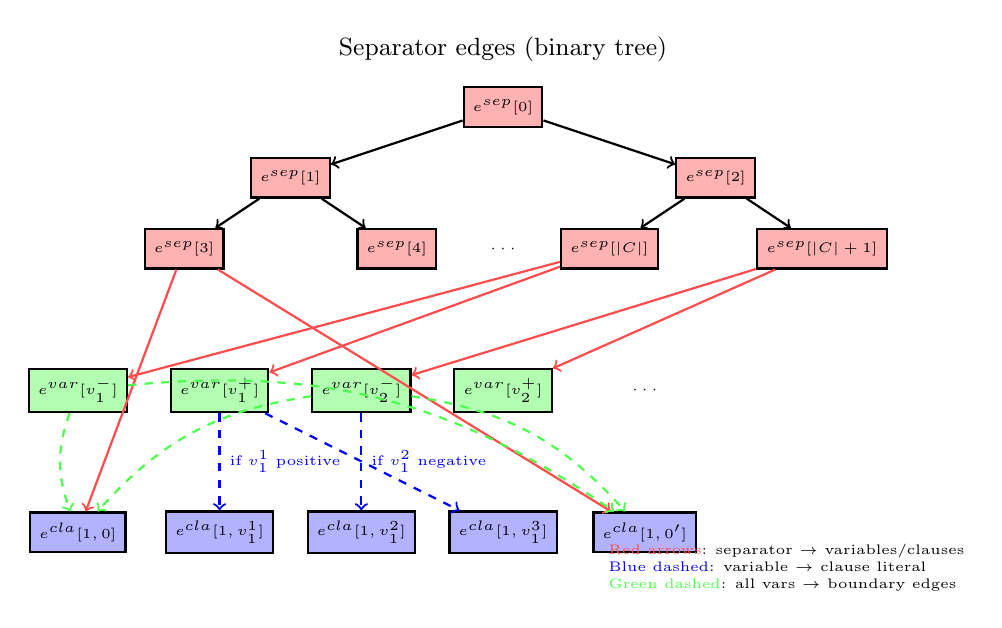
\begin{tikzpicture}[scale=0.9]
    % Define node styles
    \tikzstyle{sepnode}=[rectangle, fill=red!30, draw=black, thick, minimum size=5mm, font=\tiny]
    \tikzstyle{varnode}=[rectangle, fill=green!30, draw=black, thick, minimum size=5mm, font=\tiny]
    \tikzstyle{clanode}=[rectangle, fill=blue!30, draw=black, thick, minimum size=5mm, font=\tiny]
    
    % Top level: Separator edges (binary tree structure)
    \node[sepnode] (sep0) at (6, 5) {$e^{sep}[0]$};
    
    \node[sepnode] (sep1) at (3, 4) {$e^{sep}[1]$};
    \node[sepnode] (sep2) at (9, 4) {$e^{sep}[2]$};
    
    \node[sepnode] (sep3) at (1.5, 3) {$e^{sep}[3]$};
    \node[sepnode] (sep4) at (4.5, 3) {$e^{sep}[4]$};
    \node at (6, 3) {\tiny $\cdots$};
    \node[sepnode] (sep5) at (7.5, 3) {$e^{sep}[|C|]$};
    \node[sepnode] (sep6) at (10.5, 3) {$e^{sep}[|C|+1]$};
    
    % Draw separator tree
    \draw[->, thick] (sep0) -- (sep1);
    \draw[->, thick] (sep0) -- (sep2);
    \draw[->, thick] (sep1) -- (sep3);
    \draw[->, thick] (sep1) -- (sep4);
    \draw[->, thick] (sep2) -- (sep5);
    \draw[->, thick] (sep2) -- (sep6);
    
    \node[above, font=\small] at (6, 5.5) {Separator edges (binary tree)};
    
    % Middle level: Variable edges
    \node[varnode] (var1m) at (0, 1) {$e^{var}[v_1^-]$};
    \node[varnode] (var1p) at (2, 1) {$e^{var}[v_1^+]$};
    \node[varnode] (var2m) at (4, 1) {$e^{var}[v_2^-]$};
    \node[varnode] (var2p) at (6, 1) {$e^{var}[v_2^+]$};
    \node at (8, 1) {\tiny $\cdots$};
    
    % Arrows from separators to variables
    \draw[->, thick, red!70] (sep5) -- (var1m);
    \draw[->, thick, red!70] (sep5) -- (var1p);
    \draw[->, thick, red!70] (sep6) -- (var2m);
    \draw[->, thick, red!70] (sep6) -- (var2p);
    
    % Bottom level: Clause edges
    \node[clanode] (cla10) at (0, -1) {$e^{cla}[1,0]$};
    \node[clanode] (cla1v1) at (2, -1) {$e^{cla}[1,v_1^1]$};
    \node[clanode] (cla1v2) at (4, -1) {$e^{cla}[1,v_1^2]$};
    \node[clanode] (cla1v3) at (6, -1) {$e^{cla}[1,v_1^3]$};
    \node[clanode] (cla10p) at (8, -1) {$e^{cla}[1,0']$};
    
    % Arrows from separators to clause boundary edges
    \draw[->, thick, red!70] (sep3) -- (cla10);
    \draw[->, thick, red!70] (sep3) -- (cla10p);
    
    % Arrows from variables to clause literal edges (precedence constraints)
    \draw[->, thick, blue, dashed] (var1p) -- node[right, font=\tiny] {if $v_1^1$ positive} (cla1v1);
    \draw[->, thick, blue, dashed] (var2m) -- node[right, font=\tiny] {if $v_1^2$ negative} (cla1v2);
    \draw[->, thick, blue, dashed] (var1p) -- (cla1v3);
    
    % Arrows from all variables to boundary edges
    \draw[->, thick, green!70, dashed] (var1m) to[bend right=20] (cla10);
    \draw[->, thick, green!70, dashed] (var2m) to[bend right=20] (cla10);
    \draw[->, thick, green!70, dashed] (var1m) to[bend left=20] (cla10p);
    \draw[->, thick, green!70, dashed] (var2m) to[bend left=20] (cla10p);
    
    % Legend
    \node[align=left, font=\tiny] at (10, -1.5) {
        \textcolor{red!70}{Red arrows}: separator $\to$ variables/clauses\\
        \textcolor{blue}{Blue dashed}: variable $\to$ clause literal\\
        \textcolor{green!70}{Green dashed}: all vars $\to$ boundary edges
    };
    
\end{tikzpicture}
